\documentclass{article}

% If you're new to LaTeX, here's some short tutorials:
% https://www.overleaf.com/learn/latex/Learn_LaTeX_in_30_minutes
% https://en.wikibooks.org/wiki/LaTeX/Basics

% Formatting
\usepackage{subfig}
\usepackage{hyperref}
\usepackage{subcaption}
\usepackage[utf8]{inputenc}
\usepackage[margin=1in]{geometry}
\usepackage[titletoc,title]{appendix}

% Math
% https://www.overleaf.com/learn/latex/Mathematical_expressions
% https://en.wikibooks.org/wiki/LaTeX/Mathematics
\usepackage{amsmath,amsfonts,amssymb,mathtools}

% Images
% https://www.overleaf.com/learn/latex/Inserting_Images
% https://en.wikibooks.org/wiki/LaTeX/Floats,_Figures_and_Captions
\usepackage{graphicx,float}

% Tables
% https://www.overleaf.com/learn/latex/Tables
% https://en.wikibooks.org/wiki/LaTeX/Tables

% Algorithms
% https://www.overleaf.com/learn/latex/algorithms
% https://en.wikibooks.org/wiki/LaTeX/Algorithms
\usepackage[ruled,vlined]{algorithm2e}
\usepackage{algorithmic}

% Code syntax highlighting
% https://www.overleaf.com/learn/latex/Code_Highlighting_with_minted
\usepackage{minted}
\usemintedstyle{borland}

% References
% https://www.overleaf.com/learn/latex/Bibliography_management_in_LaTeX
% https://en.wikibooks.org/wiki/LaTeX/Bibliography_Management
\usepackage{biblatex}
\addbibresource{references.bib}

% Title content
\title{
    \textbf{CSE343: Machine Learning} \\ \vspace*{-5pt}
    \textbf{\large{Assignment-1}}
}

\author{\href{mailto:shubham21099@iiitd.ac.in}{Shubham Sharma (2021099)}}
\date{\today}

\geometry{a4paper, left=20mm, right=20mm, top=20mm, bottom=20mm}

\begin{document}

\maketitle

% Abstract
% \begin{abstract}
%     Add your abstract here.
% \end{abstract}

% Introduction and Overview
\section{Section A (Theoretical)}
% Add your introduction and overview here.

% Example Subsection
\subsection*{Solution (a)}
\begin{figure}[h] % h = here, t = top, b = bottom, etc.
    \centering
    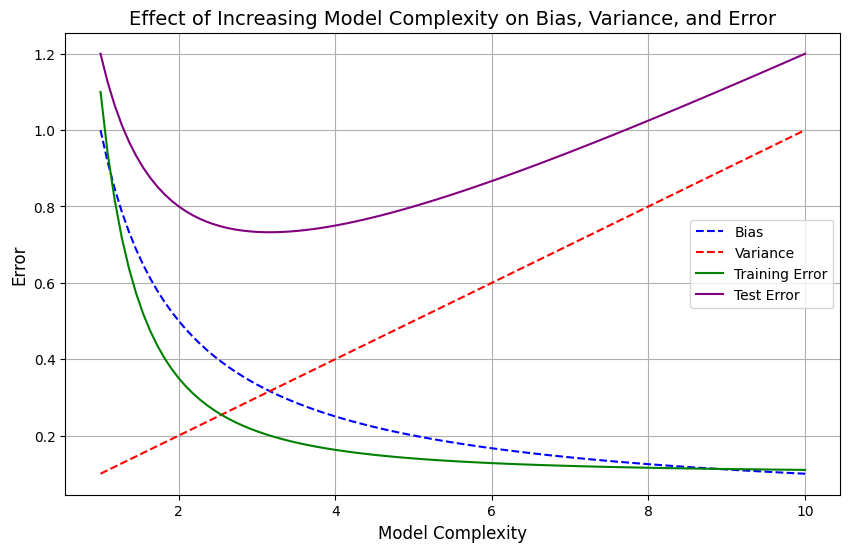
\includegraphics[width=0.5\linewidth]{assets/Aa.png}
    \caption{Bias vs Variance}
    \label{fig:a}
\end{figure}
As model complexity increases by adding more features or higher-order polynomial terms, bias decreases because the model becomes more flexible and can better fit the training data and outliers. This will lead to overfitting and hence reduce the bias. However, variance increases as the model starts fitting both the true patterns and the noise in the training data. Consequently, the model becomes highly sensitive to small changes in the training set, performing well on the training data but generalizing poorly to unseen data.

\vspace{10pt}
\subsection*{Solution (b)}
We will calculate the overall classification performance using metrics such as: Accuracy, Precision, Recall, and F1 score.
\begin{itemize}
    \item True Positives (TP) = 200
    \item False Negatives (FN) = 50
    \item True Negatives (TN) = 730
    \item False Positives (FP) = 20
\end{itemize}

\subsubsection*{Accuracy}
\[
\text{Accuracy} = \frac{TP + TN}{TP + TN + FP + FN}
\]
\[
\text{Accuracy} = \frac{200 + 730}{200 + 730 + 20 + 50} = \frac{930}{1000} = 0.93 \text{ or } 93\%
\]

\subsubsection*{Precision}
\[
\text{Precision} = \frac{TP}{TP + FP}
\]
\[
\text{Precision} = \frac{200}{200 + 20} = \frac{200}{220} = 0.909 \text{ or } 90.9\%
\]

\subsubsection*{Recall}
\[
\text{Recall} = \frac{TP}{TP + FN}
\]
\[
\text{Recall} = \frac{200}{200 + 50} = \frac{200}{250} = 0.8 \text{ or } 80\%
\]

\subsubsection*{F1 Score}
\[
F1 = 2 \times \frac{\text{Precision} \times \text{Recall}}{\text{Precision} + \text{Recall}}
\]
\[
F1 = 2 \times \frac{0.909 \times 0.8}{0.909 + 0.8} = 2 \times \frac{0.7272}{1.709} \approx 0.851 \text{ or } 85.1\%
\]
\vspace{1pt}
\hspace{-5pt}
These metrics suggest that the model has high precision, meaning that most emails flagged as spam are indeed spam. However, the recall is lower, indicating that some spam emails are missed. The overall performance, as indicated by the F1 score, is reasonably strong.


\vspace{10pt}
\subsection*{Solution (c)}
\subsubsection*{Step 1: Calculate Necessary Sums}

We need to calculate $x_i^2$ and $x_i \cdot y_i$ for each $x_i$ and $y_i$:

\[
\begin{array}{|c|c|c|c|}
\hline
x_i & y_i & x_i^2 & x_i \cdot y_i \\
\hline
3 & 15 & 9 & 45 \\
6 & 30 & 36 & 180 \\
10 & 55 & 100 & 550 \\
15 & 85 & 225 & 1275 \\
18 & 100 & 324 & 1800 \\
\hline
\end{array}
\]

\subsubsection*{Step 2: Find the Sums and Means}

\hspace{15pt}Sum of $x$:
\[
\sum x_i = 3 + 6 + 10 + 15 + 18 = 52
\]

Sum of $y$:
\[
\sum y_i = 15 + 30 + 55 + 85 + 100 = 285
\]

Sum of $x^2$:
\[
\sum x_i^2 = 9 + 36 + 100 + 225 + 324 = 694
\]

Sum of $x_i \cdot y_i$:
\[
\sum x_i \cdot y_i = 45 + 180 + 550 + 1275 + 1800 = 3850
\]

Mean of $x$:
\[
\bar{x} = \frac{\sum x_i}{n} = \frac{52}{5} = 10.4
\]

Mean of $y$:
\[
\bar{y} = \frac{\sum y_i}{n} = \frac{285}{5} = 57
\]

\subsubsection*{Step 3: Calculate the Slope $a$}

The formula for the slope $a$ is:
\[
a = \frac{\frac{\sum x_i y_i}{n} - \frac{\sum x_i \cdot \sum y_i}{n^2}}{\frac{\sum x_i^2}{n} - (\frac{\sum x_i}{n})^2}
\]

Substituting the values:
\[
a = \frac{\frac{3850}{5} - \frac{52 \cdot 285}{5^2}}{\frac{694}{5} - \left( \frac{52}{5} \right)^2}
\]

\[
a = \frac{770 - 592.8}{138.8 - 108.16} = \frac{177.2}{30.64} = 5.78
\]

\subsubsection*{Step 4: Calculate the Intercept \(b\)}

The formula for the intercept \(b\) is:
\[
b = \bar{y} - a \cdot \bar{x}
\]

Substitute the values:
\[
b = 57 - 5.78 \cdot 10.4 = 57 - 60.11 = -3.11
\]

\subsubsection*{Step 5: Equation of the Regression Line}

The equation of the regression line is:
\[
y = 5.78x - 3.11
\]

\subsubsection*{Step 6: Predict the Value of \(y\) When \(x = 12\)}

Substitute \(x = 12\) into the regression equation:
\[
y = 5.78 \cdot 12 - 3.11 = 69.36 - 3.11 = 66.25
\]

\hspace{-15pt}Thus, the predicted value of $\mathbf{y}$ when $\mathbf{x = 12}$ is $\mathbf{66.25}$ units.


\vspace{10pt}
\subsection*{Solution (d)}
\subsubsection*{Toy Example}
Let's consider an example of a simple dataset, which consists of only one input feature, X, and a simple regression problem where we want to predict Y as a continuous output variable. Our training dataset consists of 10 samples, with X values ranging from 0 to 9, and corresponding Y values.
Entries in dataset is of the form like : \{\{0, 0\}, \{1, 1\}, \{2, 4\}, \{3, 9\}, .... , \{9, 81\}\}.

\subsubsection*{Model $f_1$: $$f_1(x) = a_0 + a_1x + a_2x^2 + a_3x^3 + a_4x^4 + a_5x^5 + a_6x^6 + a_7x^7 + a_8x^8 + a_9x^9$$}

\subsubsection*{Model $f_2$: $$f_2(x) = mx + c$$}

\begin{figure}[H] % h = here, t = top, b = bottom, etc.
    \centering
    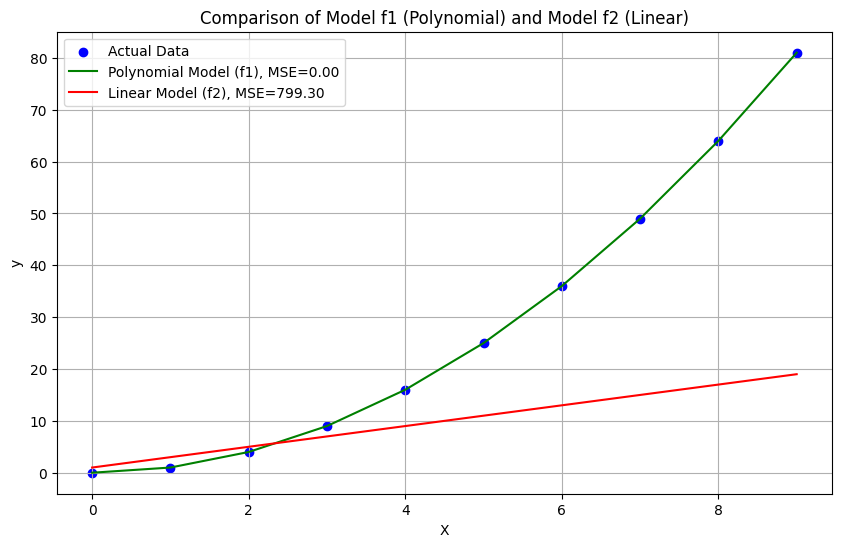
\includegraphics[width=0.5\linewidth]{assets/Ad.png}
    \caption{Empirical Risk of f1 vs f2}
    \label{fig:a}
\end{figure}

$f_1$ is a 9th-degree polynomial that perfectly fits the training data. On the other hand $f_2$ is a simple linear model. 
$f_1$ has zero empirical risk on the training set. $f_2$ has a higher empirical risk on the training set compared to $f_1$, as it doesn't perfectly fit the data.

\subsubsection*{Empirical Risk Comparison}
\begin{itemize}
\item $f_1$: Since $f_1$ perfectly fits the data, because for a dataset with n points, a polynomial of degree n-1 can perfectly fit all the data points hence its empirical risk is 0.
\item $f_2$: The empirical risk of $f_2$ can be calculated as the mean squared error (MSE) between the predicted and actual $Y$ values. After calculation, we got an empirical risk of 799.30, which is much higher than the empirical risk of f1.
\end{itemize}


\subsubsection*{Generalization}

Let $X = 13$

\begin{itemize}
\item $f_1$: For the given X $f_1$ will predict a $Y$ value that is extremely large, as it's trying to derive the trend from the training data. Because the model is too complex and does not generalize well and hence it will produce an example of overfitting.
\item $f_2$: $f_2$ is a simple linear model that will predict a more generalized value, which is a more reasonable prediction of the trend.
\end{itemize}


\vspace{50pt} % add 10pt of vertical space
\section{Section B (Scratch Implementation)}
\subsection*{Solution (a)}
\subsubsection*{Convergence of the Model}
\begin{figure}[H] % h = here, t = top, b = bottom, etc.
    \centering
    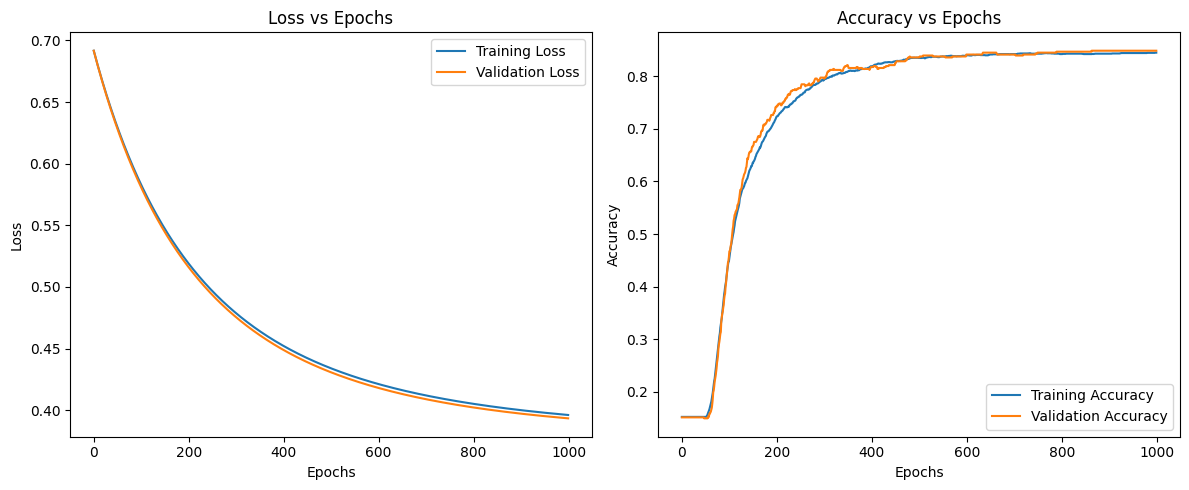
\includegraphics[width=0.5\linewidth]{assets/a.png}
    \caption{Loss vs Epochs and Accuracy vs Epochs}
    \label{fig:a}
\end{figure}
\hspace{-3pt}
From the graphs, we can observe that for $\alpha = 0.01$ and 1000 epochs, our loss is constantly decreasing with each iteration, and our accuracy is increasing with each iteration. Also, the model is converged quickly at around 700 iterations. And performing well on training and validation set. (I applied standard scaling just only for this (a) part)

\vspace{20pt}
\subsection*{Solution (b)}
\subsubsection*{Feature Scaling}
\begin{figure}[H] % h = here, t = top, b = bottom, etc.
    \centering
    \begin{minipage}{0.49\linewidth}
        \centering
        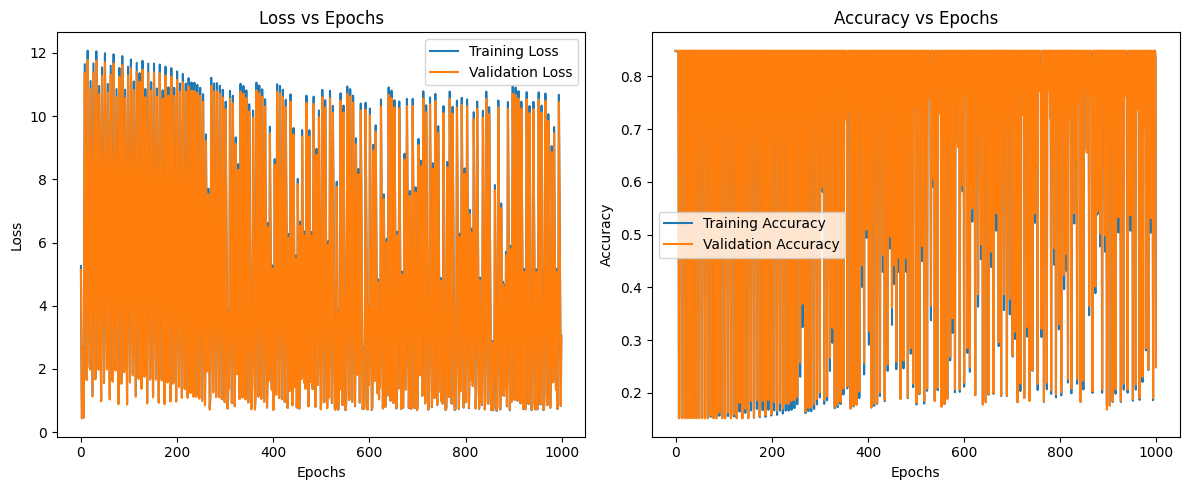
\includegraphics[width=\linewidth]{assets/b-1.png}
        \caption{Without Scaling}{}
        \label{fig:b-1}
    \end{minipage}
    \hfill
    \begin{minipage}{0.49\linewidth}
        \centering
        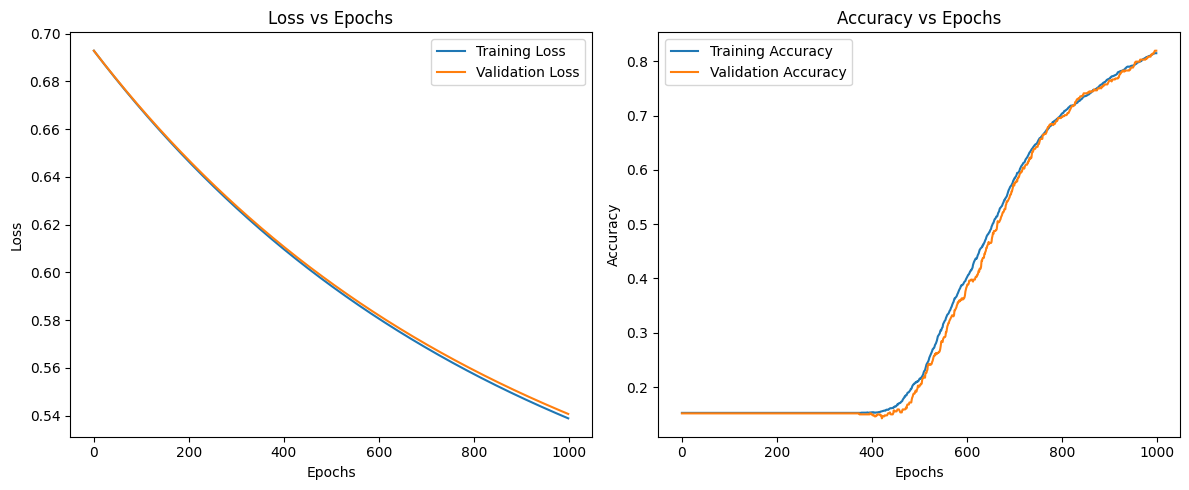
\includegraphics[width=\linewidth]{assets/b-2.png}
        \caption{With Min-Max Scaling}{}
        \label{fig:b-2}
    \end{minipage}
\end{figure}
\hspace{-3pt}
From the above two graphs we can conclude that without any scaling the model is performing very poorly and both loss and acuracy are very fluctuating and model is also not converging. But after applying "min-max" scaling the model is performing very well, both loss and accuracy are constantly decreasing and increasing respectively with each iteration and finally model get converged also.

\vspace{30pt}
\subsection*{Solution (c)}
\subsubsection*{Insights from Metrics}
\begin{figure}[h]
    \centering
    \begin{minipage}[c]{0.45\linewidth}
        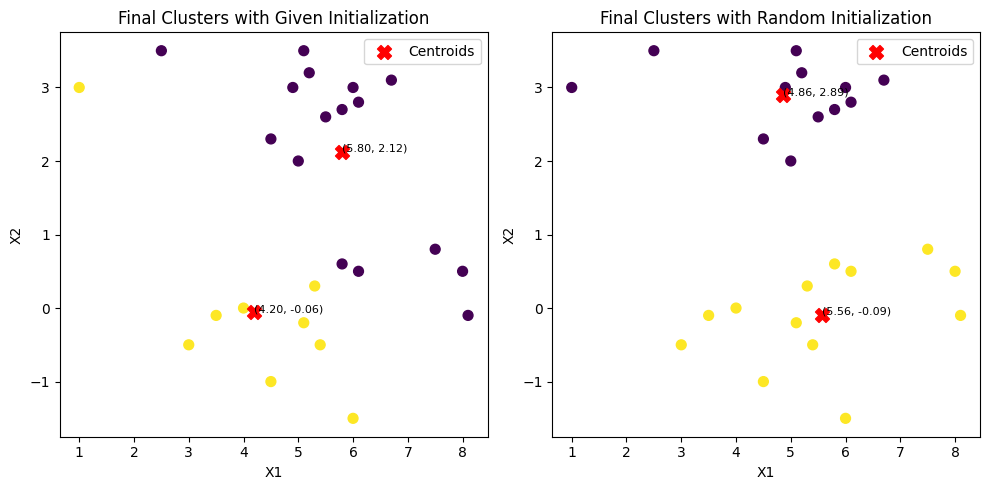
\includegraphics[width=\linewidth]{assets/c.png}
        \caption{Confusion Matrix}
        \label{fig:a}
    \end{minipage}
    \begin{minipage}[c]{0.45\linewidth}
        \centering
        \vspace{0.5cm}
        \begin{tabular}{|l|c|}
            \hline
            Metric & Value \\ \hline
            Precision & 0.0556 \\ \hline
            Recall & 0.0119 \\ \hline
            F1 Score & 0.0196 \\ \hline
            ROC-AUC Score & 0.3110 \\ \hline
        \end{tabular}
        \captionof{table}{Observations}
    \end{minipage}
\end{figure}

\begin{enumerate}
\item The model shows very poor performance in identifying the positive class, as reflected by the very low recall (1.2\%) and precision (5.56\%). This indicates class imbalance, where the negative class dominates the dataset, causing the model to focus on predicting negatives.
\item With 82 false negatives, the model is missing most of the actual positive instances.
\item Low ROC-AUC and F1 Scores also indicate the imbalance of classes in the dataset.
\end{enumerate}

\vspace{10pt}
\subsection*{Solution (d)}
\subsubsection*{Comparison of different Optimisation Algorithms}
\vspace{10pt}
\begin{figure}[H] % h = here, t = top, b = bottom, etc.
    \centering
    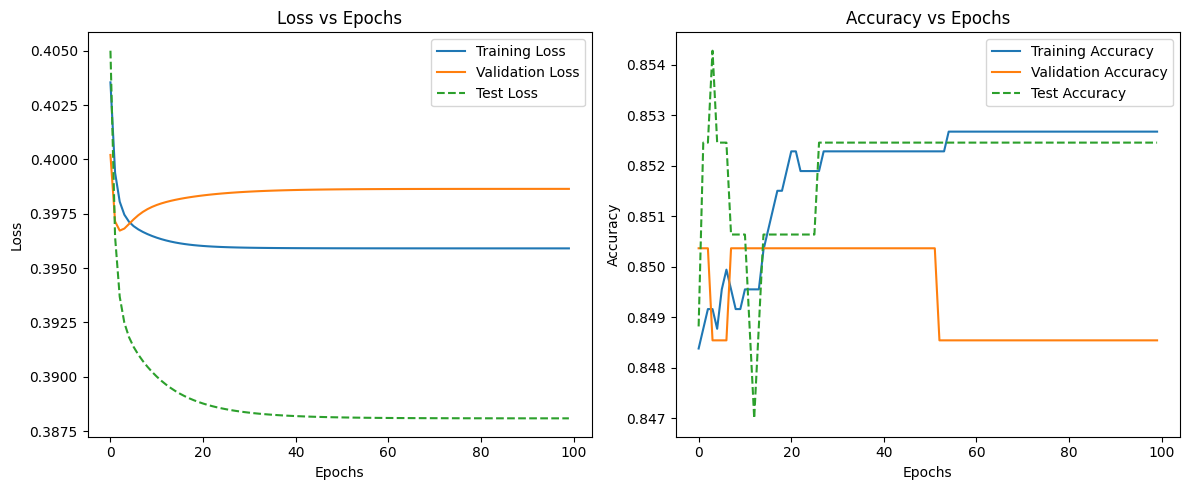
\includegraphics[width=0.5\linewidth]{assets/d-SGD.png}
    \caption{SGD}
    \label{fig:a}
\end{figure}
\begin{figure}[H] % h = here, t = top, b = bottom, etc.
    \centering
    \begin{minipage}{0.49\linewidth}
        \centering
        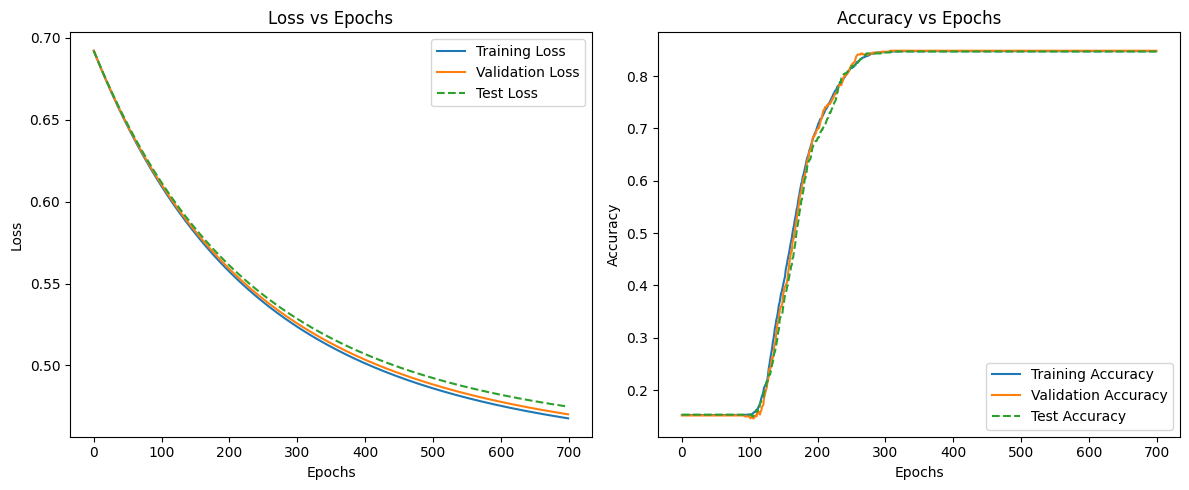
\includegraphics[width=\linewidth]{assets/d-MBGD-64.png}
        \caption{MBGD-64}{}
        \label{fig:b-1}
    \end{minipage}
    \hfill
    \begin{minipage}{0.49\linewidth}
        \centering
        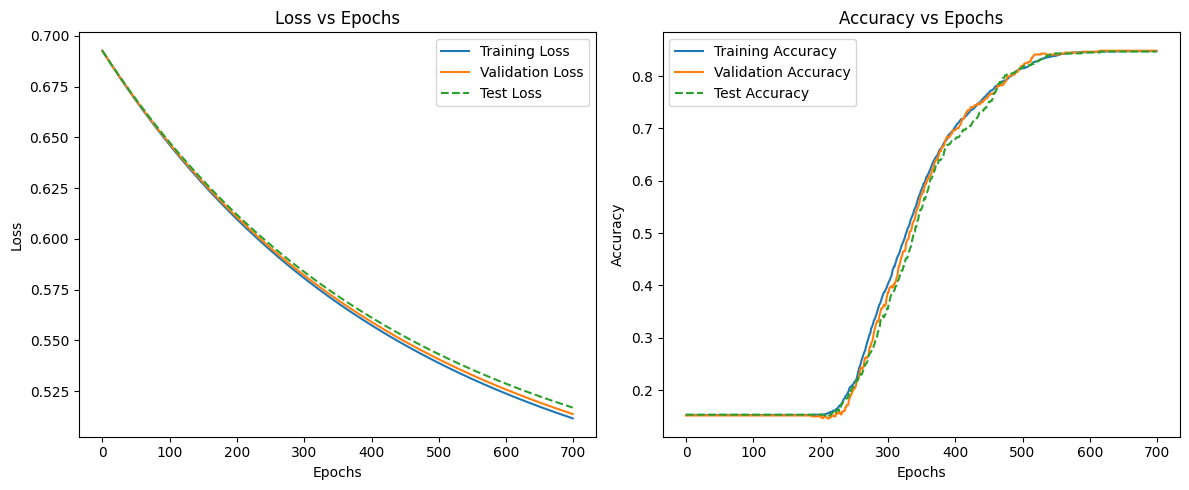
\includegraphics[width=\linewidth]{assets/d-MBGD-128.png}
        \caption{MBGD-128}{}
        \label{fig:b-2}
    \end{minipage}
\end{figure}
% \vspace*{80pt}
\hspace{0pt}From the above three pairs of graphs, i.e., Stochastic Gradient Descent (SGD), Mini-Batch Gradient Descent-64 (MBGD-64), and Mini-Batch Gradient Descent-128 (MBGD-128), we come to the following conclusions:

\begin{enumerate}
\item SGD converges fast as compared to others because it performs more updates in a single iteration.
\item As compared to SGD, both MBGD-64 and MBGD-128 have much smoother convergence.
\item For the same number of iterations and learning rate, MBGD-64 took fewer iterations to converge compared to MBGD-128 due to its smaller batch size.
\item In terms of stability, MBGD-128 is much more stable than the other two.
\end{enumerate}

\vspace{10pt}
\subsection*{Solution (e)}
\subsubsection*{Analysis of K-fold Cross-Validation}

\begin{figure}[H] % h = here, t = top, b = bottom, etc.
    \centering
    \begin{minipage}{0.49\linewidth}
        \centering
        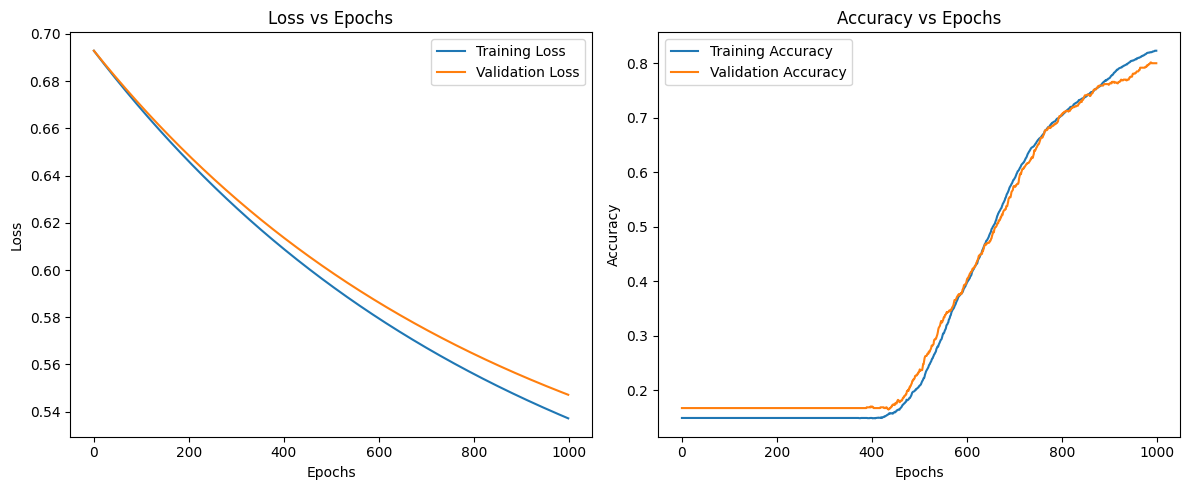
\includegraphics[width=\linewidth]{assets/e-f1.png}
        \caption{Fold 1}{}
        \label{fig:b-1}
    \end{minipage}
    \hfill
    \begin{minipage}{0.49\linewidth}
        \centering
        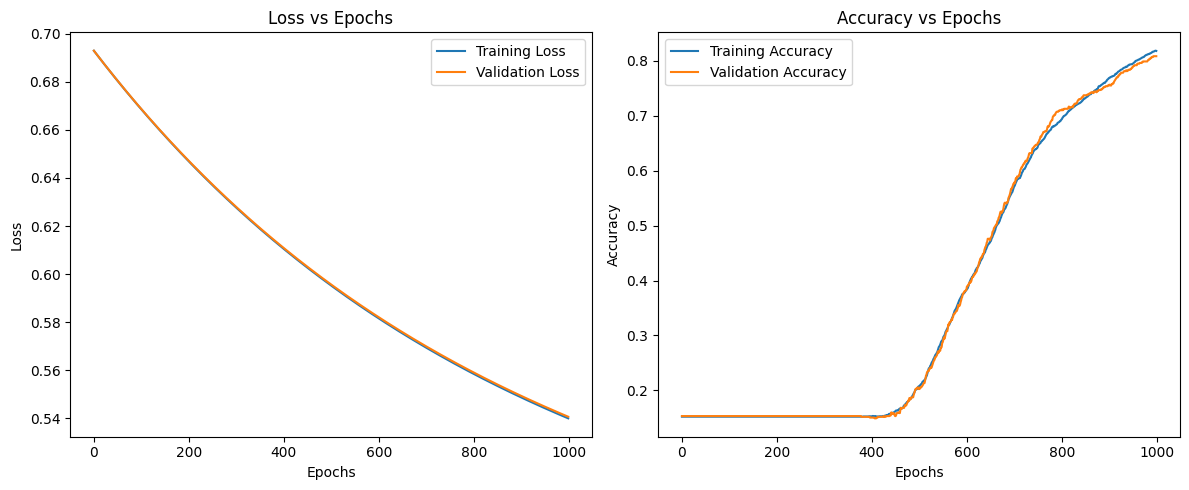
\includegraphics[width=\linewidth]{assets/e-f2.png}
        \caption{Fold 2}{}
        \label{fig:b-2}
    \end{minipage}
\end{figure}

\begin{figure}[H] % h = here, t = top, b = bottom, etc.
    \centering
    \begin{minipage}{0.49\linewidth}
        \centering
        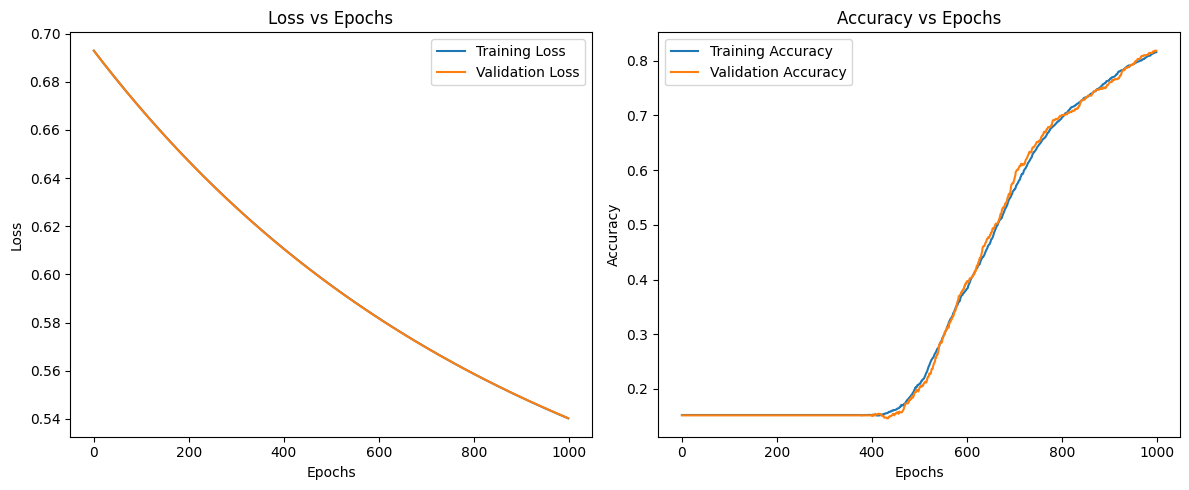
\includegraphics[width=\linewidth]{assets/e-f3.png}
        \caption{Fold 3}{}
        \label{fig:b-1}
    \end{minipage}
    \hfill
    \begin{minipage}{0.49\linewidth}
        \centering
        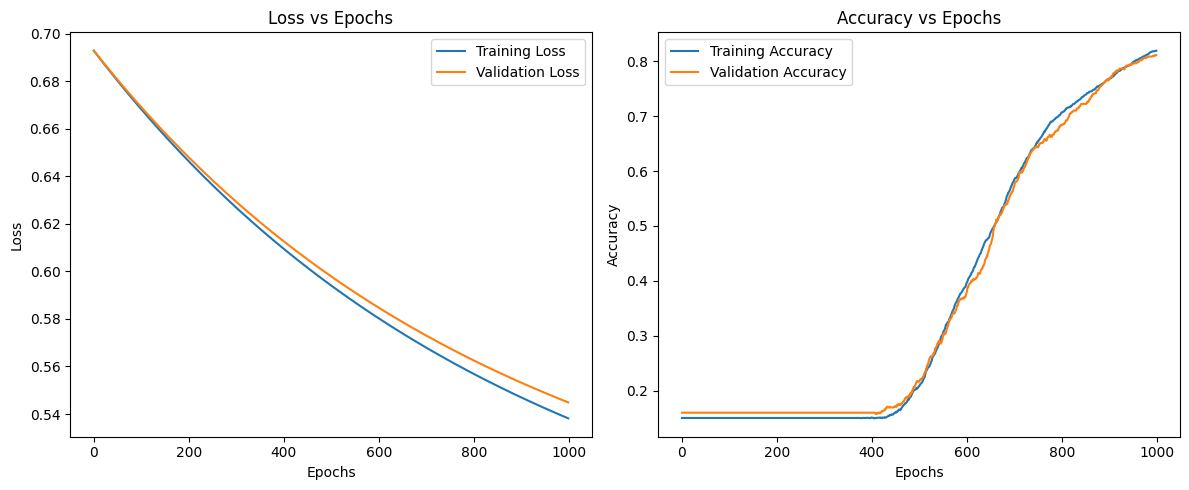
\includegraphics[width=\linewidth]{assets/e-f4.png}
        \caption{Fold 4}{}
        \label{fig:b-2}
    \end{minipage}
\end{figure}

\begin{figure}[H]
    \centering
    \begin{minipage}[c]{0.45\linewidth}
        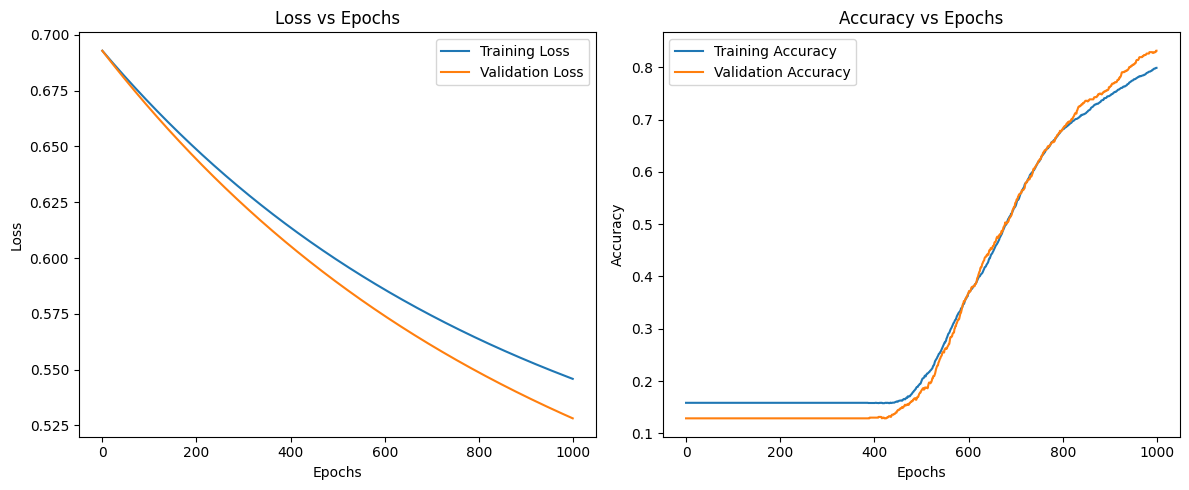
\includegraphics[width=\linewidth]{assets/e-f5.png}
        \caption{Fold 5}
        \label{fig:a}
    \end{minipage}
    \begin{minipage}[c]{0.45\linewidth}
        \centering
        \vspace{0.5cm}
        \begin{tabular}{|l|c|c|}
            \hline
            Metric & Mean & Std \\ \hline
            Accuracy & 0.8140 & 0.0106 \\ \hline
            Precision & 0.0325 & 0.0399 \\ \hline
            Recall & 0.0100 & 0.0130 \\ \hline
            F1 Score & 0.0151 & 0.0193 \\ \hline
        \end{tabular}
        \captionof{table}{Average Results (k=5)}
    \end{minipage}
\end{figure}

\hspace{-3pt}
From the Graph and average of metrics we can conclude that the model's performance is relatively stable and consistent across different folds, with low variances and small standard deviations. This suggests that the model is robust and can generalize well to new, unseen data.

% \clearpage % This ensures the page break happens here

\vspace{10pt}
\subsection*{Solution (f)}
\subsubsection*{Early Stopping and its Effect of Overfitting and Generalization}
\begin{figure}[H] % h = here, t = top, b = bottom, etc.
    \centering
    \begin{minipage}{0.49\linewidth}
        \centering
        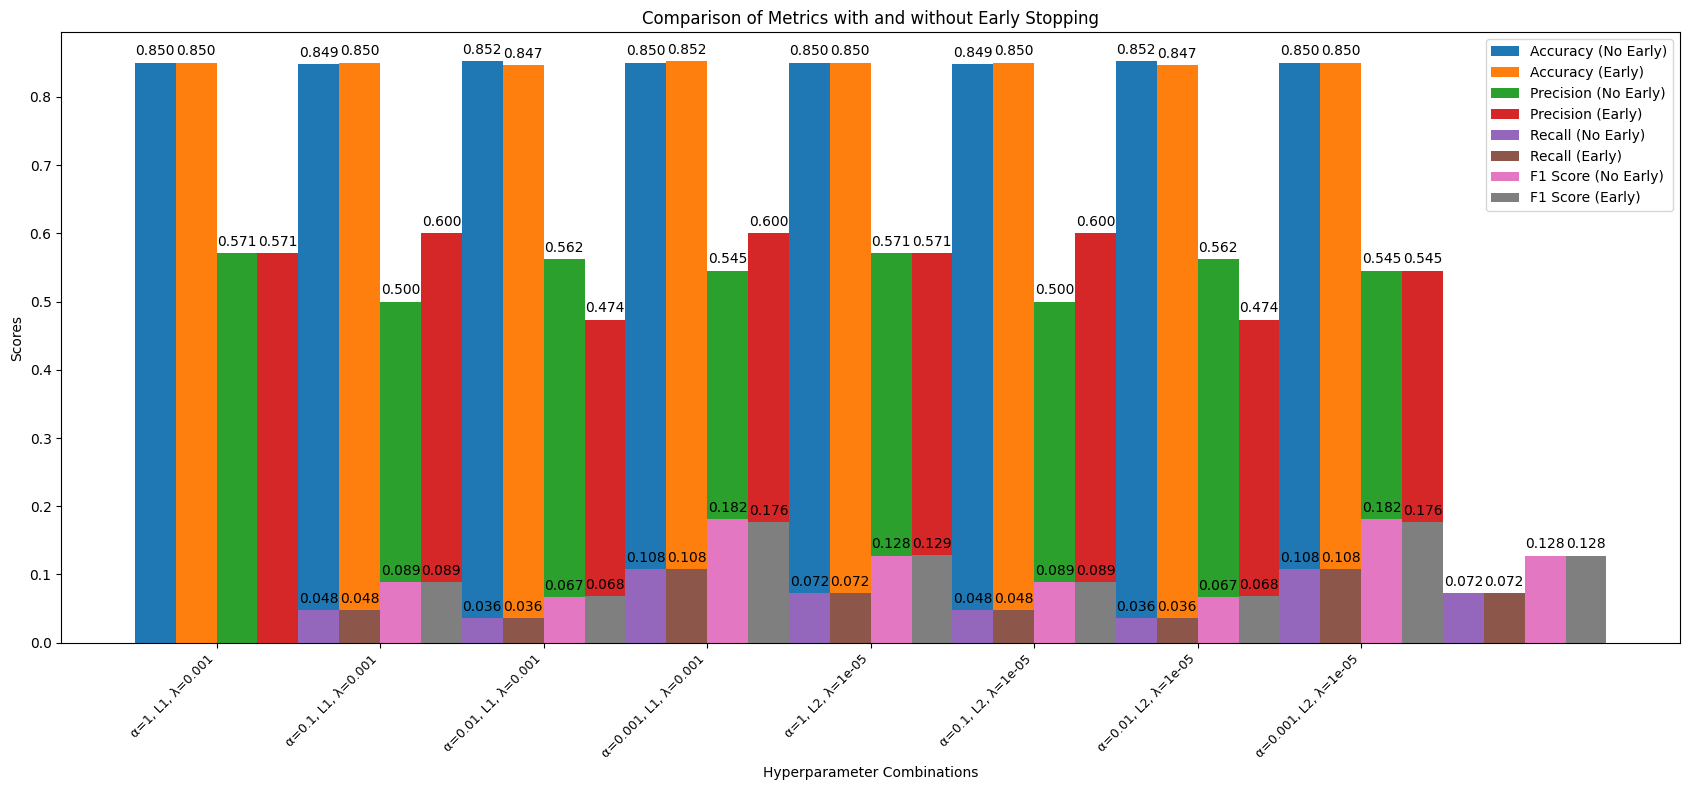
\includegraphics[width=\linewidth]{assets/fV.png}
        \caption{Validation Dataset}{}
        \label{fig:b-1}
    \end{minipage}
    \hfill
    \begin{minipage}{0.49\linewidth}
        \centering
        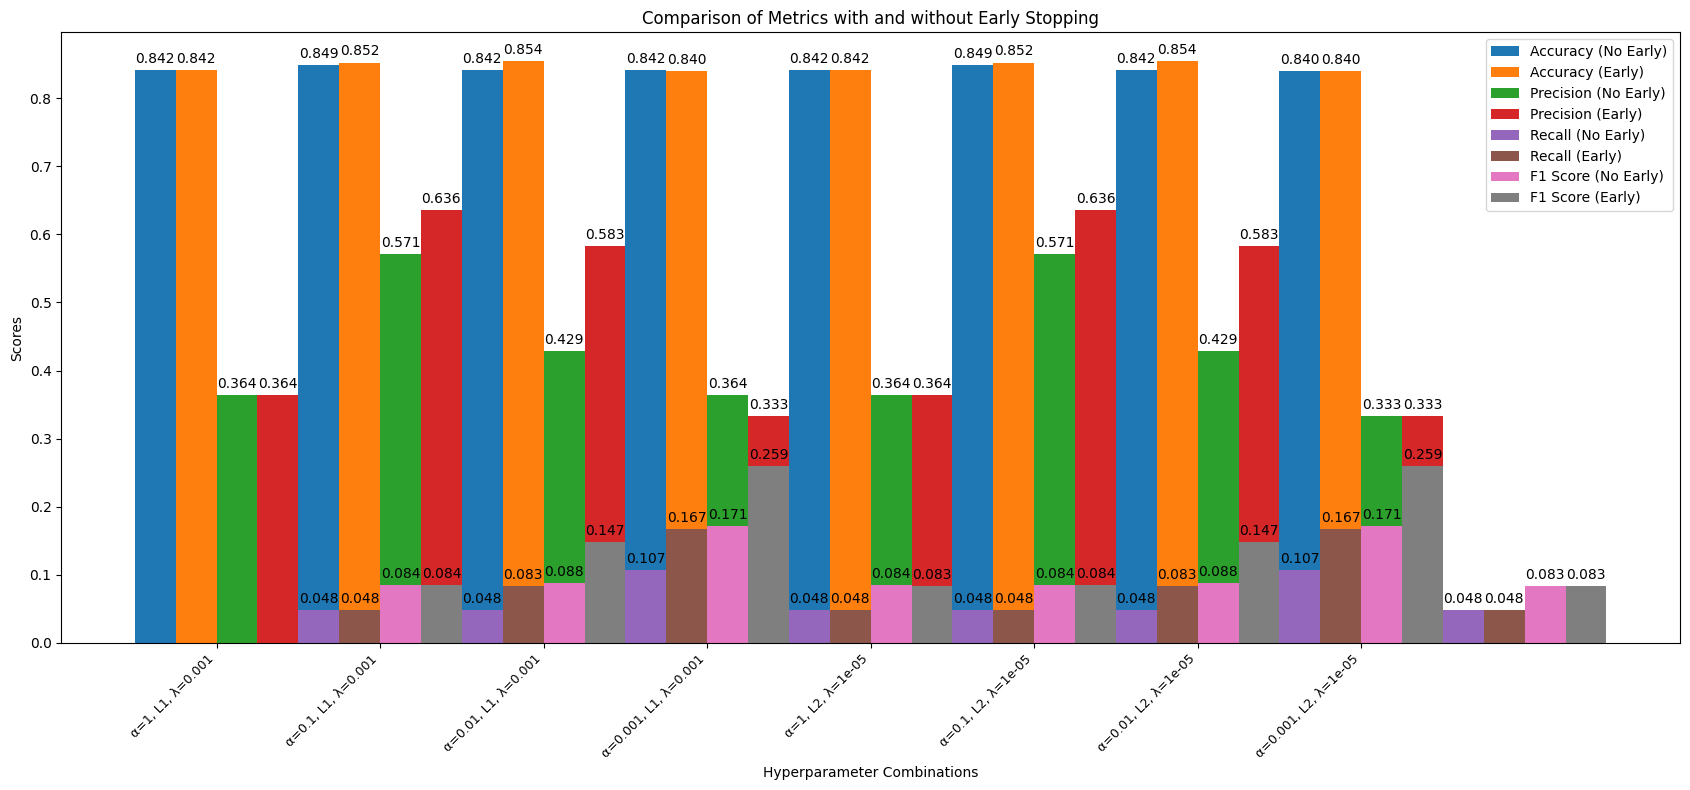
\includegraphics[width=\linewidth]{assets/fT.png}
        \caption{Test Dataset}{}
        \label{fig:b-2}
    \end{minipage}
    \caption*{Comparing impact of Early Stopping \& No Early Stopping}
\end{figure}

\hspace{-20pt}
\begin{table}[H]
\centering
\resizebox{\textwidth}{!}{
\begin{tabular}{|c|c|c|c|c|c|c|}
\hline
$\alpha$ & Regularization & $\lambda$ & Accuracy (ES/NO-ES) & Precision (ES/NO-ES) & Recall (ES/NO-ES) & F1 (ES/NO-ES) \\ 
\hline
1     & L1  & 0.001  & (0.8415, 0.8415) & (0.3636, 0.3636) & (0.0476, 0.0476) & (0.0842, 0.0842) \\ \hline
0.1   & L1  & 0.001  & (0.8525, 0.8488) & (0.6364, 0.5714) & (0.0833, 0.0476) & (0.1474, 0.0879) \\ \hline
0.01  & L1  & 0.001  & (0.8543, 0.8415) & (0.5833, 0.4286) & (0.1667, 0.1071) & (0.2593, 0.1714) \\ \hline
0.001 & L1  & 0.001  & (0.8397, 0.8415) & (0.3333, 0.3636) & (0.0476, 0.0476) & (0.0833, 0.0842) \\ \hline
1     & L2  & 1e-05  & (0.8415, 0.8415) & (0.3636, 0.3636) & (0.0476, 0.0476) & (0.0842, 0.0842) \\ \hline
0.1   & L2  & 1e-05  & (0.8525, 0.8488) & (0.6364, 0.5714) & (0.0833, 0.0476) & (0.1474, 0.0879) \\ \hline
0.01  & L2  & 1e-05  & (0.8543, 0.8415) & (0.5833, 0.4286) & (0.1667, 0.1071) & (0.2593, 0.1714) \\ \hline
0.001 & L2  & 1e-05  & (0.8397, 0.8397) & (0.3333, 0.3333) & (0.0476, 0.0476) & (0.0833, 0.0833) \\ 
\hline
\end{tabular}
}
\caption{Comparison of Early Stopping (ES) and No Early Stopping (NO-ES).}
\end{table}



\hspace{-15pt}To prevent overfitting, I choose the early stopping parameter as patience = 10 and min\_delta = 1e-3. This means that training will stop if the validation loss does not improve by at least 1e-3 for 10 consecutive epochs.
\vspace{5pt}
\newline\hspace{-15pt}After trying eight different combinations of learning rate ($\alpha$) = \{1, 0.1, 0.01, 0.001\} and L1, L2 regularization, I come to the conclusion that early stopping stops the overfitting and promotes the generalization of the unseen test data. As it will be clearly visible in the metrics data. From all combinations of models in which early stopping is enabled, has better accuracy, precision, recall, and F1-score.

\end{document}
